\section{Introduction}\label{sec:introduction}

Some citation \cite{dodelson2020modern} and \cite{weinberg2008cosmology}

Also write about the following:

\begin{itemize}
    \item Cosmological principle
    \item Einstein field equation
    \item Homogeneity and isotropy
    \item FLRW metric 
\end{itemize}

In order to explain the connection between spacetime itself and the energy distribution within it we must solve the Einstein equation:
\begin{equation}\label{eq:introduction:einstein_equation}
    G_\munu = 8\pi GT_\munu,
\end{equation}
where $G_\munu$ is the Einstein tensor describing the geometry of spacetime, $G$ is the gravitational constant and $T_\munu$ is the energy and momentum tensor.

\begin{figure}
    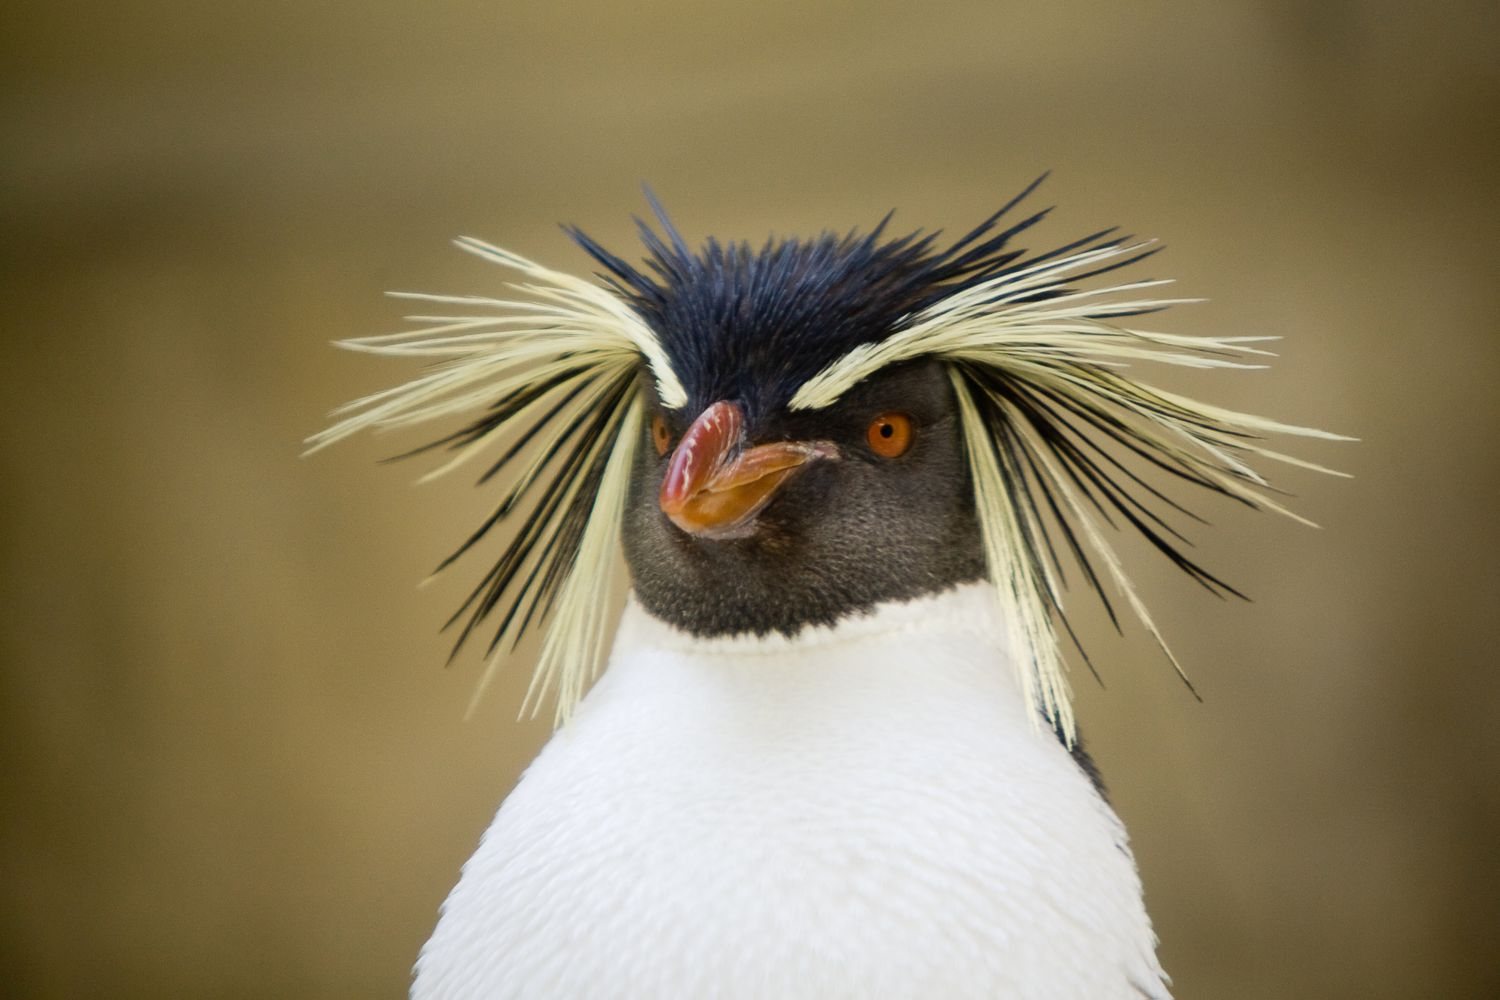
\includegraphics[width=\linewidth]{penguin.jpg}
    \label{fig:penguin}
    \caption{Penguin making sure that you do all the work necessary!}
\end{figure}